\section{Castle of Dynamia}

\begin{figure}[H]
  \centering
  \includegraphics[width=\textwidth]{Images/Maps/castleOfDynamiaPuzzles}
  \caption{Puzzles locations in the Castle of Dynamia}
\end{figure}

%\subsection{1. Build the Spider machine}
%
%%\begin{figure}[H]
%%  \centering
%%  \includegraphics[width=\textwidth]{Images/Puzzles/castleOfDynamia_1}
%%  \caption{Puzzle 1 in the Castle of Dynamia}
%%\end{figure}
%
%In order to enter in the courtyard, the player can use some debris to build the Spider machine that allows him/her to climb the wall without being detected.
%
%\textit{This puzzle is alternative to a fight.}
%
%%The player has different parts and he/she has to understand how to combine them. He/She has to break some part to obtain new components. Some parts are not required to build the machine.
%
%%The player has to reorder the pieces of a mosaic representing the machine itself.
%%
%%The mosaic has 4 rows and 6 columns. The player can switch any couple of two pieces.
%
%%\subsubsection*{Hints}
%%If the player gets stuck for some time, Sophie will tell some lines to help the player, at the same time two pieces will be highlighted in order to suggest to switch them.
%%
%%\textbf{Sophie}: I think that piece should go there.
%
%See the section \textit{Machine building puzzle}.

\subsection{1. Distract the guard}

Pick up the glass bottle on the ground and throw it away to distract the guard, than sneak in undetected while he moves away from the gate.

\textit{This puzzle is alternative to a fight.}


\subsection{2. Rotate the torch}

\begin{figure}[H]
  \centering
  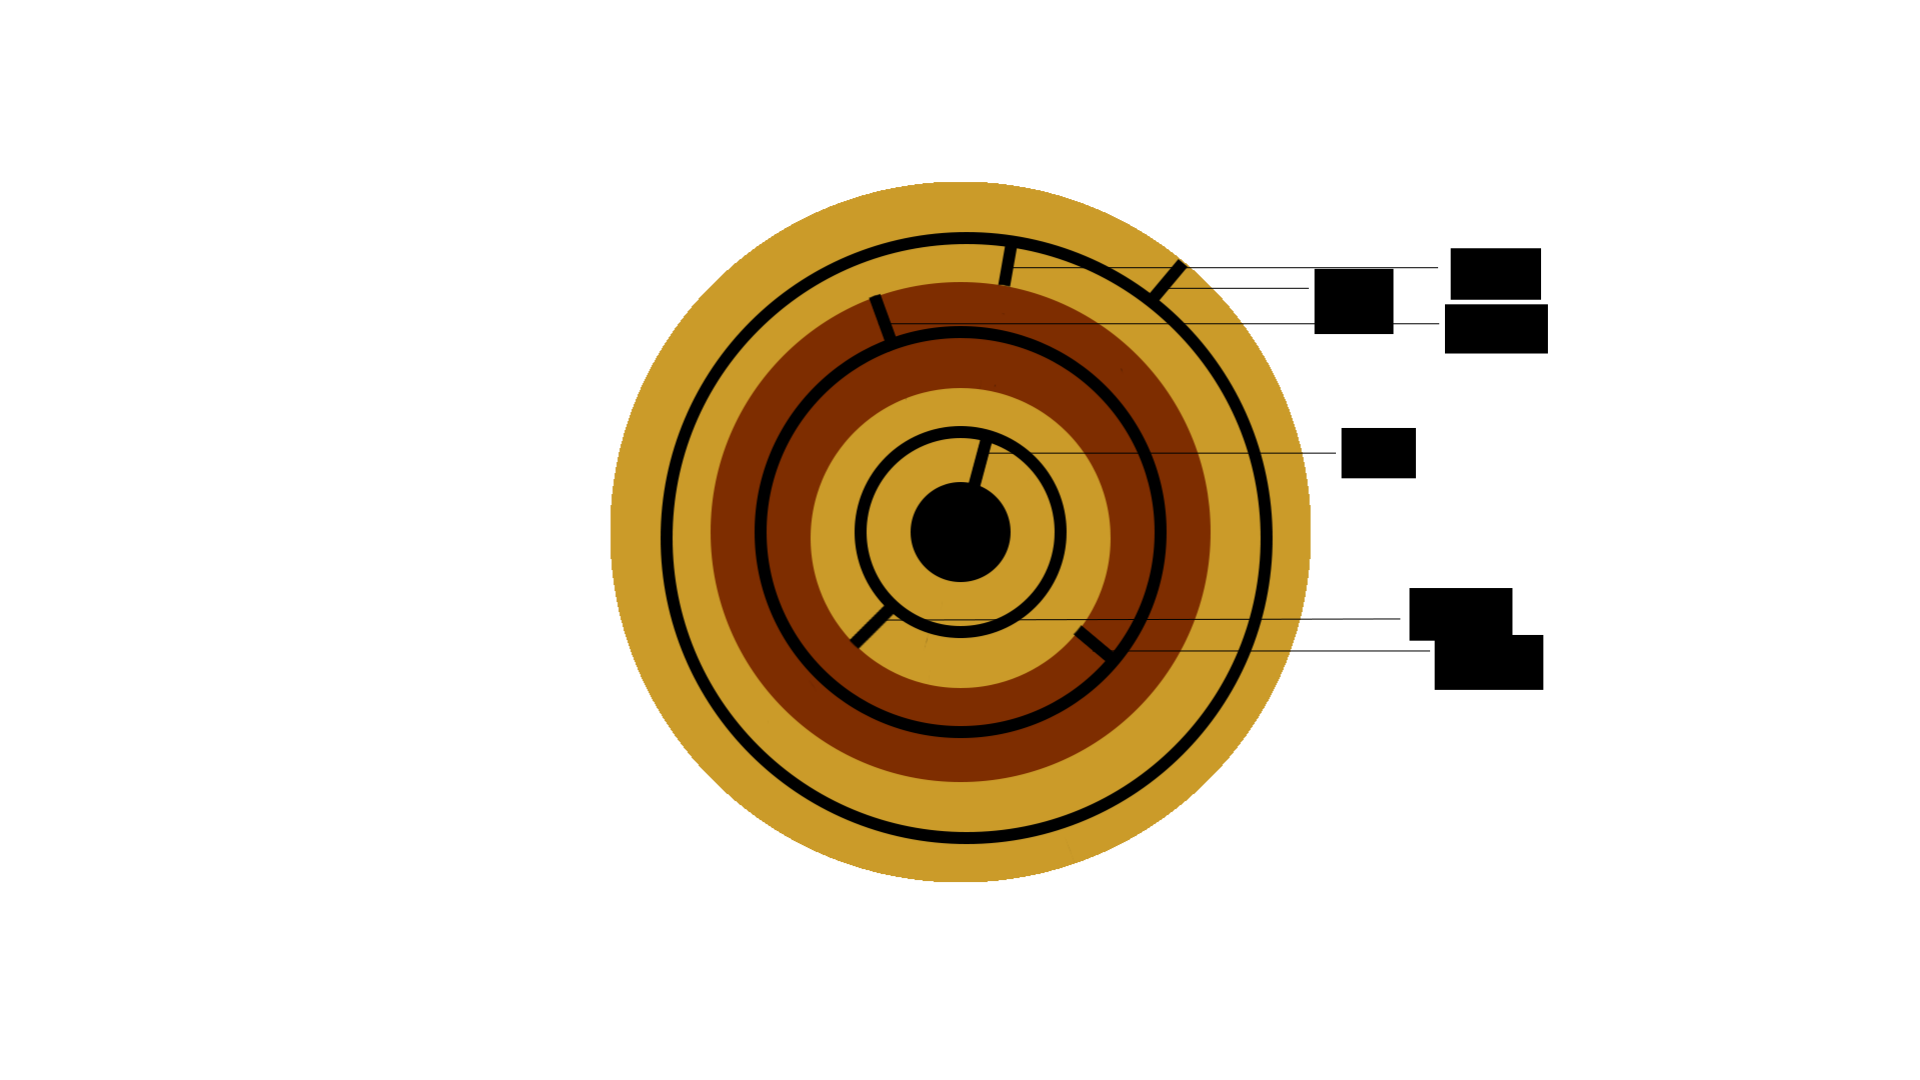
\includegraphics[width=10cm]{Images/Puzzles/castleOfDynamia2}
  \caption{Puzzle 2 in the Castle of Dynamia}
\end{figure}

The player has to rotate three rings at the base of the torch in order to align them in the proper way to create an uninterrupted black path. The player can reset all of the three circles to the starting state by rotating the arm of the torch. The player is supposed to be already taught about how to play this game in the previous levels

When the player rotates the outer ring of one step, the middle ring rotates in the same direction.

When the player rotates the middle ring of one step, the outer ring rotates in the same direction.

When the player rotate the inner ring of one step, the middle ring rotates in the same direction.

\textit{This puzzle is alternative to a fight.}

\subsubsection*{Technical details}
The starting and the final position of the circles can be found in the pictures here above.

The inner circle rotates by 15 degrees and make the middle one rotate by 15 degrees for each step.

The middle circle rotates by 50 degrees and make the outer one rotate by 15 degrees for each step.

The outer circle rotates by 10 degrees and make the middle one rotate by 5 degrees for each step.

\subsubsection*{Solution}
\begin{figure}[H]
  \centering
  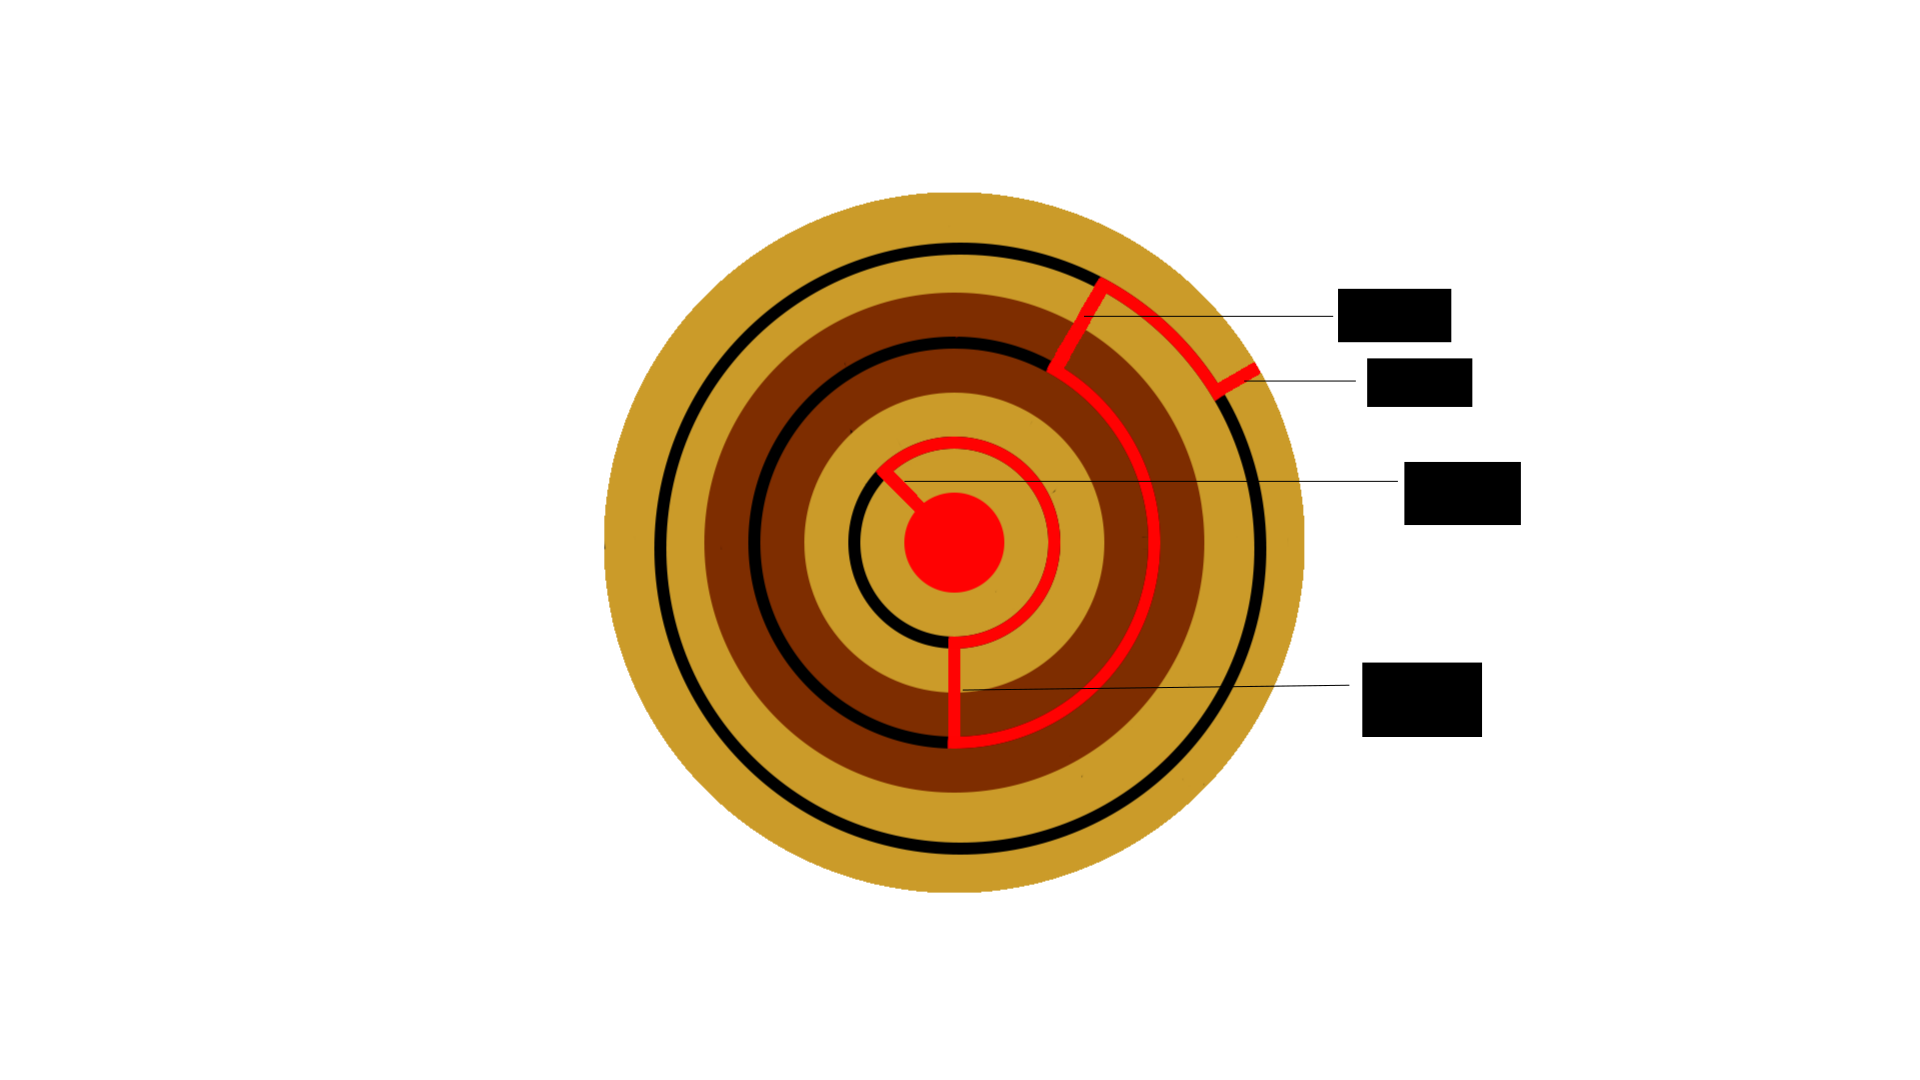
\includegraphics[width=10cm]{Images/Puzzles/castleOfDynamia2Solution}
  \caption{Solution of puzzle 2 in the Castle of Dynamia}
\end{figure}

The optimal solution is composed by three steps (that can be done in any order):
\begin{itemize}
	\item Rotate anticlockwise the inner circle by three steps.
	\item Rotate clockwise the middle circle by two steps.
	\item Rotate clockwise the outer circle by one step.
\end{itemize}

\subsubsection*{Hints}
If the player gets stuck for some time, the torch will tell some lines to help the player.

If the player has not rotated correctly any of the three circle:

\textbf{Torch \#{}1}: I think turning the rings just randomly is not a good strategy. Try to start again!

If the player rotates correctly at least one of the three circles:

\textbf{Torch \#{}1}: You are on the right track! Keep going!

If the player rotates correctly two of the three circles:

\textbf{Torch \#{}1}: You are almost done! You are so close!

Once the player has done one of the step of the solution the player will hear a sound feedback: \textbf{*CLICK*}

If the player activates the sound feedback but keeps rotating:

\textbf{Torch \#{}1}: Wait! I have heard something

or

\textbf{Torch \#{}1}: Are you sure? Listen carefully!


\subsection{3. Press the bricks}

\begin{figure}[H]
  \centering
  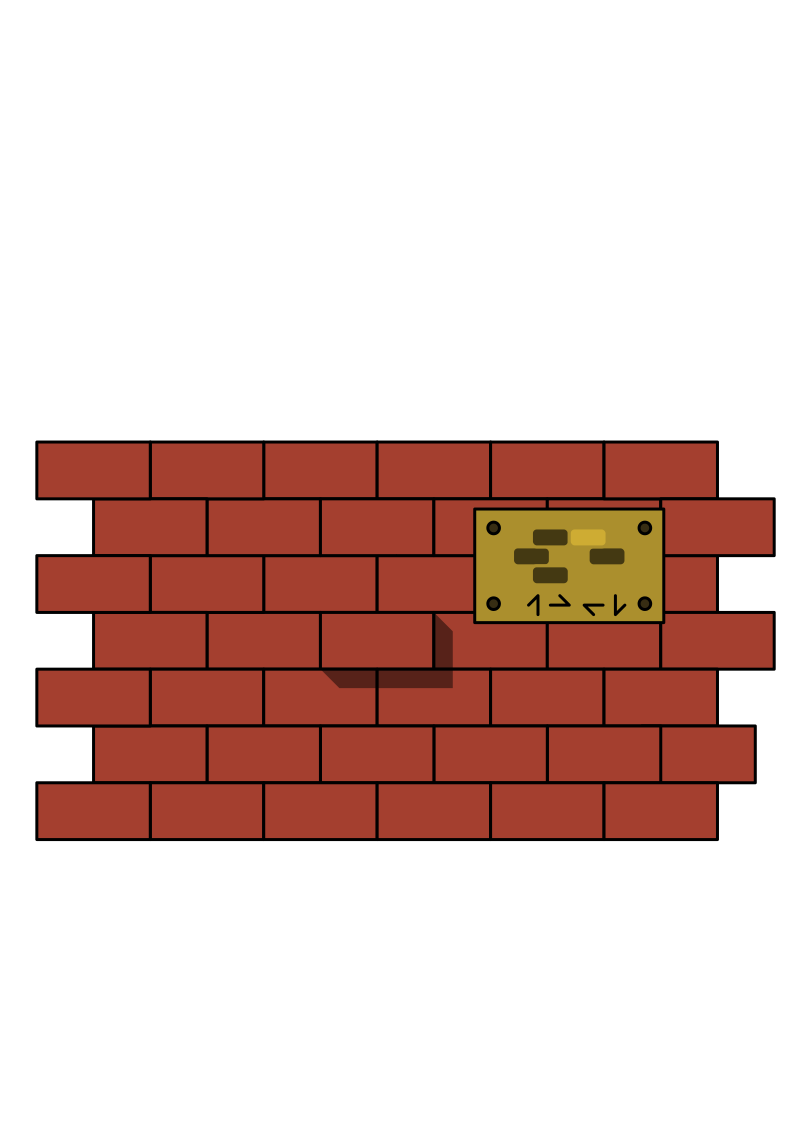
\includegraphics[width=\textwidth]{Images/Puzzles/castleOfDynamia3}
  \caption{Puzzle 3 in the Castle of Dynamia}
\end{figure}

%Near the torch there is a small plate with some horizontal lines. The player has to press the bricks in the corresponding position under the torch.

%A protruding brick helps the player to identify the bricks to press.

Under the torch there is a small rusty golden plate with four horizontal carved lines, a raised horizontal line and four small arrow

The player has to press the bricks under the torch in the positions corresponding to the carved lines. A protruding brick, corresponding to the raised line, helps the player to identify the bricks to press.

The player has to press the bricks in the order specified by the small arrows. If he/she presses them in the right order, the previous bricks stay pressed, otherwise all the bricks return to their normal state and the player has to start again.

\textit{This puzzle is alternative to a fight.}

\subsubsection*{Solution}
\begin{figure}[H]
  \centering
  \includegraphics[width=\textwidth]{Images/Puzzles/castleOfDynamia3Solution}
  \caption{Solution of the puzzle 3 in the Castle of Dynamia}
\end{figure}

\subsubsection*{Hints}
If the player gets stuck for some time, the torch will tell some lines to help the player.

\textbf{Torch \#{}2}: Four carved lines and one raise lines: it must mean something, don't it?

\textbf{Torch \#{}2}: Maybe those arrows indicate some kind of order you should follow...

%\textbf{Torch \#{}2}: Pss. You have to press the bricks in the proper order. Try to take a closer look to the plate.


\subsection{4. Connect the cables}

\begin{figure}[H]
  \centering
  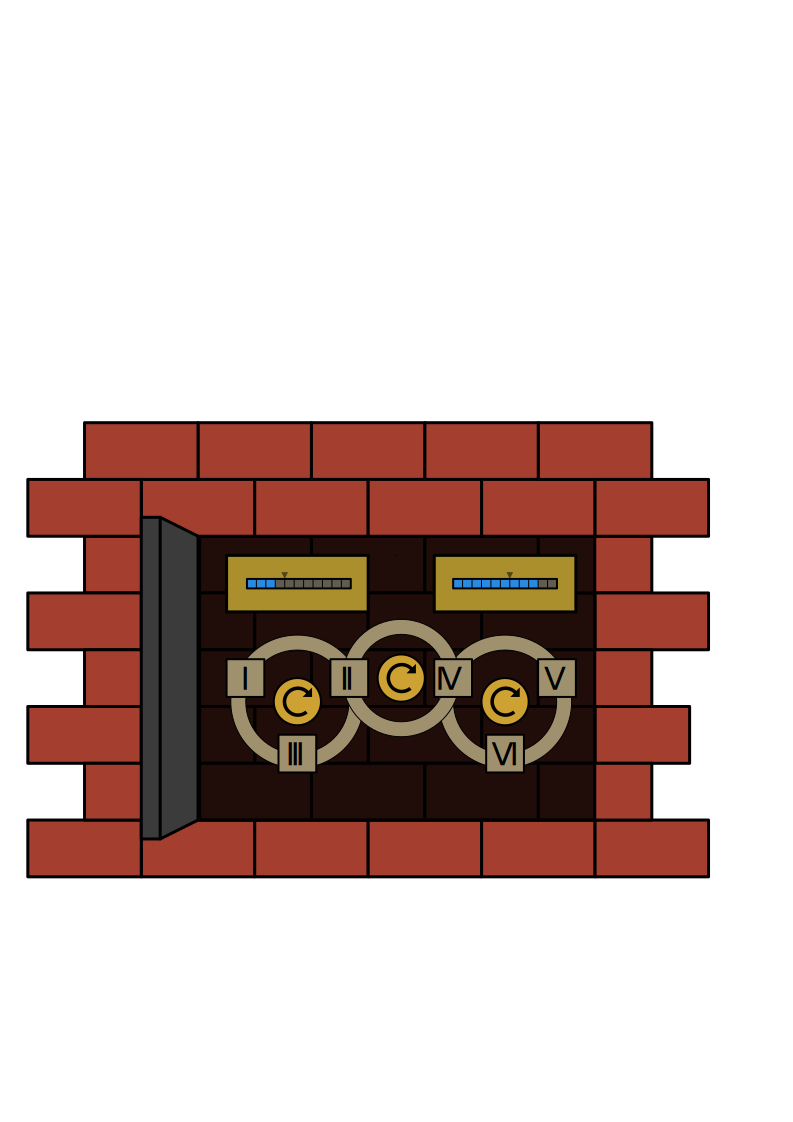
\includegraphics[width=\textwidth]{Images/Puzzles/castleOfDynamia4}
  \caption{Puzzle 4 in the Castle of Dynamia}
\end{figure}

%There are some cables that hang under the torch. The player has to connect them in the correct pairs, according to the pattern on the plugs.

Under the torch there is a metal door where there is the inscription \enquote{DO NOT TOUCH}. The player can open it and access a compartment inside the wall.

In the compartment there are three cables that hang under a small golden plate, and three terminals under another golden plate. Each plate has a bar with 5 marks. One mark per bar is highlighted: the second one on the left bar and the third one on the right bar. The bar on the left is full of a red liquid, the other one is empty.

Each plug and each terminal has a roman number.

Plugs:
\begin{itemize}
	\item I
	\item II
	\item III
\end{itemize}

Terminals:
\begin{itemize}
	\item II
	\item IV
	\item VI
\end{itemize}

The player has to connect the cables with the terminals in a way that ensure that the liquid is distributed by 2/5 on the left and 3/5 on the right.

When the player connects a plug, he/she can see some flashing lights that flow from the cable to the terminal and the bars on the plates moves according to the proportion established by the number on the plates.

\textit{Example 1 (plugs in red, terminals in blue)}
\begin{itemize}
	\item Connection: \textcolor{red}{I}-\textcolor{blue}{II}
	\item Left bar: \textcolor{red}{1}/(\textcolor{red}{1}+\textcolor{blue}{2}) = 1/3
	\item Right bar: \textcolor{blue}{2}/(\textcolor{red}{1}+\textcolor{blue}{2}) = 2/3
\end{itemize}

\textit{Examle 2 (plugs in red, terminals in blue)}
\begin{itemize}
	\item Connection: \textcolor{red}{I}-\textcolor{blue}{II} and \textcolor{red}{II}-\textcolor{blue}{IV}
	\item Left bar: (\textcolor{red}{1}+\textcolor{red}{2})/(\textcolor{red}{1}+\textcolor{blue}{2}+\textcolor{red}{2}+\textcolor{blue}{4}) = 3/9 = 1/3
	\item Right bar: (\textcolor{blue}{2}+\textcolor{blue}{4})/(\textcolor{red}{1}+\textcolor{blue}{2}+\textcolor{red}{2}+\textcolor{blue}{4}) = 6/9 = 2/3
\end{itemize}

\textit{This puzzle is alternative to a fight.}

\subsubsection*{Solution}
The player has to connect the cables I and III with the terminals II and IV (pairs are not relevant) to fill the left bar for 2/5 and the right bar for 3/5.

So the possible solutions are (plugs in red, terminals in blue):
\begin{itemize}
	\item Connection: \textcolor{red}{I}-\textcolor{blue}{II} and \textcolor{red}{III}-\textcolor{blue}{IV}
	\item Left bar: (\textcolor{red}{1}+\textcolor{red}{3})/(\textcolor{red}{1}+\textcolor{blue}{2}+\textcolor{red}{3}+\textcolor{blue}{4}) = 4/10 = 2/5
	\item Right bar: (\textcolor{blue}{2}+\textcolor{blue}{4})/(\textcolor{red}{1+\textcolor{blue}{2}}+\textcolor{red}{3}+\textcolor{blue}{4}) = 6/10 = 3/5
\end{itemize}

\begin{itemize}
	\item Connection: \textcolor{red}{I}-\textcolor{blue}{IV} and \textcolor{red}{III}-\textcolor{blue}{II}
	\item Left bar: (\textcolor{red}{1}+\textcolor{red}{3})/(\textcolor{red}{1}+\textcolor{blue}{4}+\textcolor{red}{3}+\textcolor{blue}{2}) = 4/10 = 2/5
	\item Right bar: (\textcolor{blue}{2}+\textcolor{blue}{4})/(\textcolor{red}{1}+\textcolor{blue}{4}+\textcolor{red}{3}+\textcolor{blue}{2}) = 6/10 = 3/5
\end{itemize}

\subsubsection*{Hints}
If the player gets stuck for some time, the torch will tell some lines to help the player.

\textbf{Torch \#{}3}: Maths and proportions: young people today don't really study them.

\textbf{Torch \#{}3} Maybe the numbers and the liquid are related... but how? 


\subsection{5. Stun the captain}

\begin{figure}[H]
  \centering
  \includegraphics[width=\textwidth]{Images/Puzzles/castleOfDynamia5}
  \caption{Sketch of the crumbling bricks and the two supports}
\end{figure}

In order to defeat the captain without facing him, the player can make some crumbling bricks falling on his head.

To do so, the player has to destroy two supports with Calcifer's ranged attack. Calcifer can hit only one of them when he is near the entrance to the courtyard (5A in the map), and the other one when he is near the door to the prison (5B in the map).

The player has also to draw the captain under the crumbling blocks before destroying the second support. To do so, he/she can use a bottle (5C in the map).

If the captain sees the player, he/she has to fight and defeat him.

\textit{This puzzle is alternative to a fight.}

\subsubsection*{Solution}
\begin{enumerate}
	\item Destroy the nearest support when you are near the entrance to the courtyard.
	\item Hide in the vegetation while the captain is alerted.
	\item Steal the bottle on the table in the courtyard while the captain is looking somewhere else.
	\item Go next to the door to the prison using the vegetation to hide yourself.
	\item Throw the bottle at the wall under the crumbling bricks.
	\item Wait for the captain to be under the crumbling bricks.
	\item Destroy the second support.
\end{enumerate}
